\chapter{Context}\label{chap2}

\section{Institutional Framework}
This six-month internship was conducted at the \textbf{Laboratoire Ville Mobilité Transport (LVMT)}, a research unit affiliated with \textbf{École nationale des ponts et chaussées (ENPC)}, with funding provided by the \textbf{Energy4Climate interdisciplinary center (E4C)}. This institutional arrangement reflects the collaborative nature of contemporary energy and mobility research to address complex challenges in sustainable transportation infrastructure. The following sections detail the structure, missions, and research orientations of these three interconnected organizations that provided the framework for this research project.

\textbf{ENPC} represents one of France's most prestigious engineering institutions. Founded in 1747 by Daniel-Charles Trudaine, ENPC is among the oldest French Grandes Écoles, historically focused on training engineering officials and civil engineers. The school has evolved to offer wide-ranging education including computer science, applied mathematics, civil engineering, mechanics, finance, economics, innovation, urban studies, environment and transport engineering. In July 2024, ENPC became the sixth member school of Institut Polytechnique de Paris (IP Paris), joining École polytechnique, ENSTA Paris, ENSAE Paris, Télécom Paris and Télécom SudParis.
Located on the Champs-sur-Marne campus, ENPC maintains a strong international presence with 43\% of its students obtaining double degrees abroad and 30\% of the engineering cohort being international students. The institution's research excellence is supported by 12 research laboratories, covering domains crucial to ecological, digital, and energy transitions, positioning it as a key player in addressing contemporary sustainability challenges.

\textbf{LVMT} serves as the direct host institution for this research project. Created in 2003, this multidisciplinary research laboratory operates as a joint research unit between Université Gustave Eiffel and École nationale des ponts et chaussées. Celebrating its 20th anniversary in 2023, LVMT brings together nearly 90 researchers in social sciences and engineering sciences, with expertise spanning economics, anthropology, sociology, geography, urban planning, technical economics, mathematical modeling, and computer science.
The laboratory's scientific objective centers on understanding and modeling interactions between mobility practices, transport infrastructure, and spatial organization and development. Research activities are organized around four thematic axes: mobility practices and urban access; territorial dynamics and public action; city-transport interactions; and economic analysis and transport modeling. 

\textbf{E4C} provides the funding framework and broader research context for this internship. Launched in June 2019 by IP Paris and ENPC, E4C addresses energy transition through research, training, and innovation. The center gathers 21 laboratories from Institut Polytechnique de Paris and 5 associated laboratories from ENPC, creating a unique interdisciplinary platform for energy and climate research.
Nearly 30 laboratories work within E4C on four cross-cutting themes designed to reduce greenhouse gas emissions, improve energy efficiency, deploy renewable energy, and propose relevant energy policies. The center combines diverse scientific disciplines including social and economic sciences, materials sciences and engineering, applied mathematics, computer science, and geophysics.

\section{Research Supervision and Project Continuity}

\subsection{Research Supervision Team}

This internship project was conducted under the joint supervision of two tutors, 
reflecting the interdisciplinary nature of digital twin technologies and their 
application to energy mobility systems.

\textbf{Dr. Daphné Tuncer} is my supervisor from ENPC, specializing in 
digitalisation in the energy and mobility sectors.  Prior to joining ENPC, She spent many years in the UK Higher Education. Her research keywords include electric mobility, cyberphysical systems, data management, and applied data science.

\textbf{Dr. Georgios Bouloukakis} from Télécom SudParis, provides co-supervision with expertise in IoT/Edge-driven middleware and distributed software 
systems. He is an experienced researcher and educator with over one decade of teaching and mentoring of students, having supervised 2 postdoctoral researchers, 4 Ph.D. thesis, 4 R\&D developers and 48 bachelor/master theses. 

\subsection{Research Project Integration and Continuity}

This internship project represents a direct continuation of research within the E4C framework, 
following the work of \textbf{Niemat Khoder}. Niemat's internship focused on the 
static modeling of buildings, where she developed detailed 3D representations 
of demonstrators such as DrahiX (office building in E4C campus). Her work contributed to establishing semantic 
representations of building components and visualizing their spatial and structural organization.

On this foundation, this project expands the application area from smart buildings to electric vehicle charging infrastructure, while maintaining the core concept of semantic interoperability. Unlike Niemat's research, which focuses on static structures and visualization, this project introduces dynamic data modeling, incorporating data such as the session duration, energy consumption, and user behavior into the system model, thus providing a more comprehensive description of the system's operation.

The two projects share technical continuity in that they both use NGSI-LD as the semantic modeling standard and FIWARE as the IoT platform, thus ensuring consistency in the overall methodology of the E4C research activities. However, shifting the focus to electric vehicle charging research also requires some adjustments, such as using a time-series database like CrateDB to process energy consumption data, and developing API interfaces to support simulation and prediction functionalities. 

In this way, the project extends Niemat's static modeling approach toward more dynamic mobility 
energy systems, maintaining interoperability principles while addressing the specific challenges of 
charging infrastructure.

\section{Research Background}
The rapid transition towards sustainable mobility and low-carbon energy systems presents both opportunities and challenges for researchers and practitioners. This section reviews the key research background relevant to the internship, focusing on energy and environmental challenges in transportation, the development of electric vehicle charging infrastructure, the role of digital twin and simulation methods, and the importance of data models for semantic interoperability.

\subsection{Energy and Environment Challenges in Transport}

Transport is a central contributor to both energy use and environmental pressures. In France, it represented about 32\% of final energy consumption in 2023~\cite{IEA2025_FranceEnergy}, and around 66\% of total final consumption of oil products is attributable to transport~\cite{IEA2025_FranceOil}. It is also the largest national source of greenhouse-gas (GHG) emissions, accounting for approximately 32\% of territorial emissions in 2022, with road transport—cars and heavy vehicles—being the dominant contributors~\cite{HCC2023_GHG}.Beyond climate impacts, transport significantly contributes to local air pollution. The European Environment Agency notes persistent exposure to NO\textsubscript{2}, PM\textsubscript{2.5}, and ozone in urban areas with substantial health impacts~\cite{EEA2024_AirPollution}. 

Meeting these challenges requires a rapid shift toward low-carbon energy in transport. Electricity demand in France is projected to rise to 580-640 TWh by 2035, driven partly by electromobility; according to RTE, this scenario is feasible only with accelerated renewable deployment and smart charging strategies~\cite{RTE2023_Demand2035}. Therefore, electrifying mobility must be accompanied by a decarbonized electricity supply and effective demand-side management to deliver benefits for climate, air quality, and energy security.


\subsection{Electric Vehicles and Charging Infrastructure}

The rapid growth of electric vehicles (EVs) is transforming the transport and 
energy sectors. Global EV sales neared 14 million in 2023, accounting for 18\% of 
all new cars, with projections of around 17 million in 2024, or more than one-fifth 
of global car sales~\cite{IEA2024}. Yet the acceleration of EV adoption depends 
critically on the availability of suitable charging infrastructure.

\begin{figure}[ht!]
    \centering
    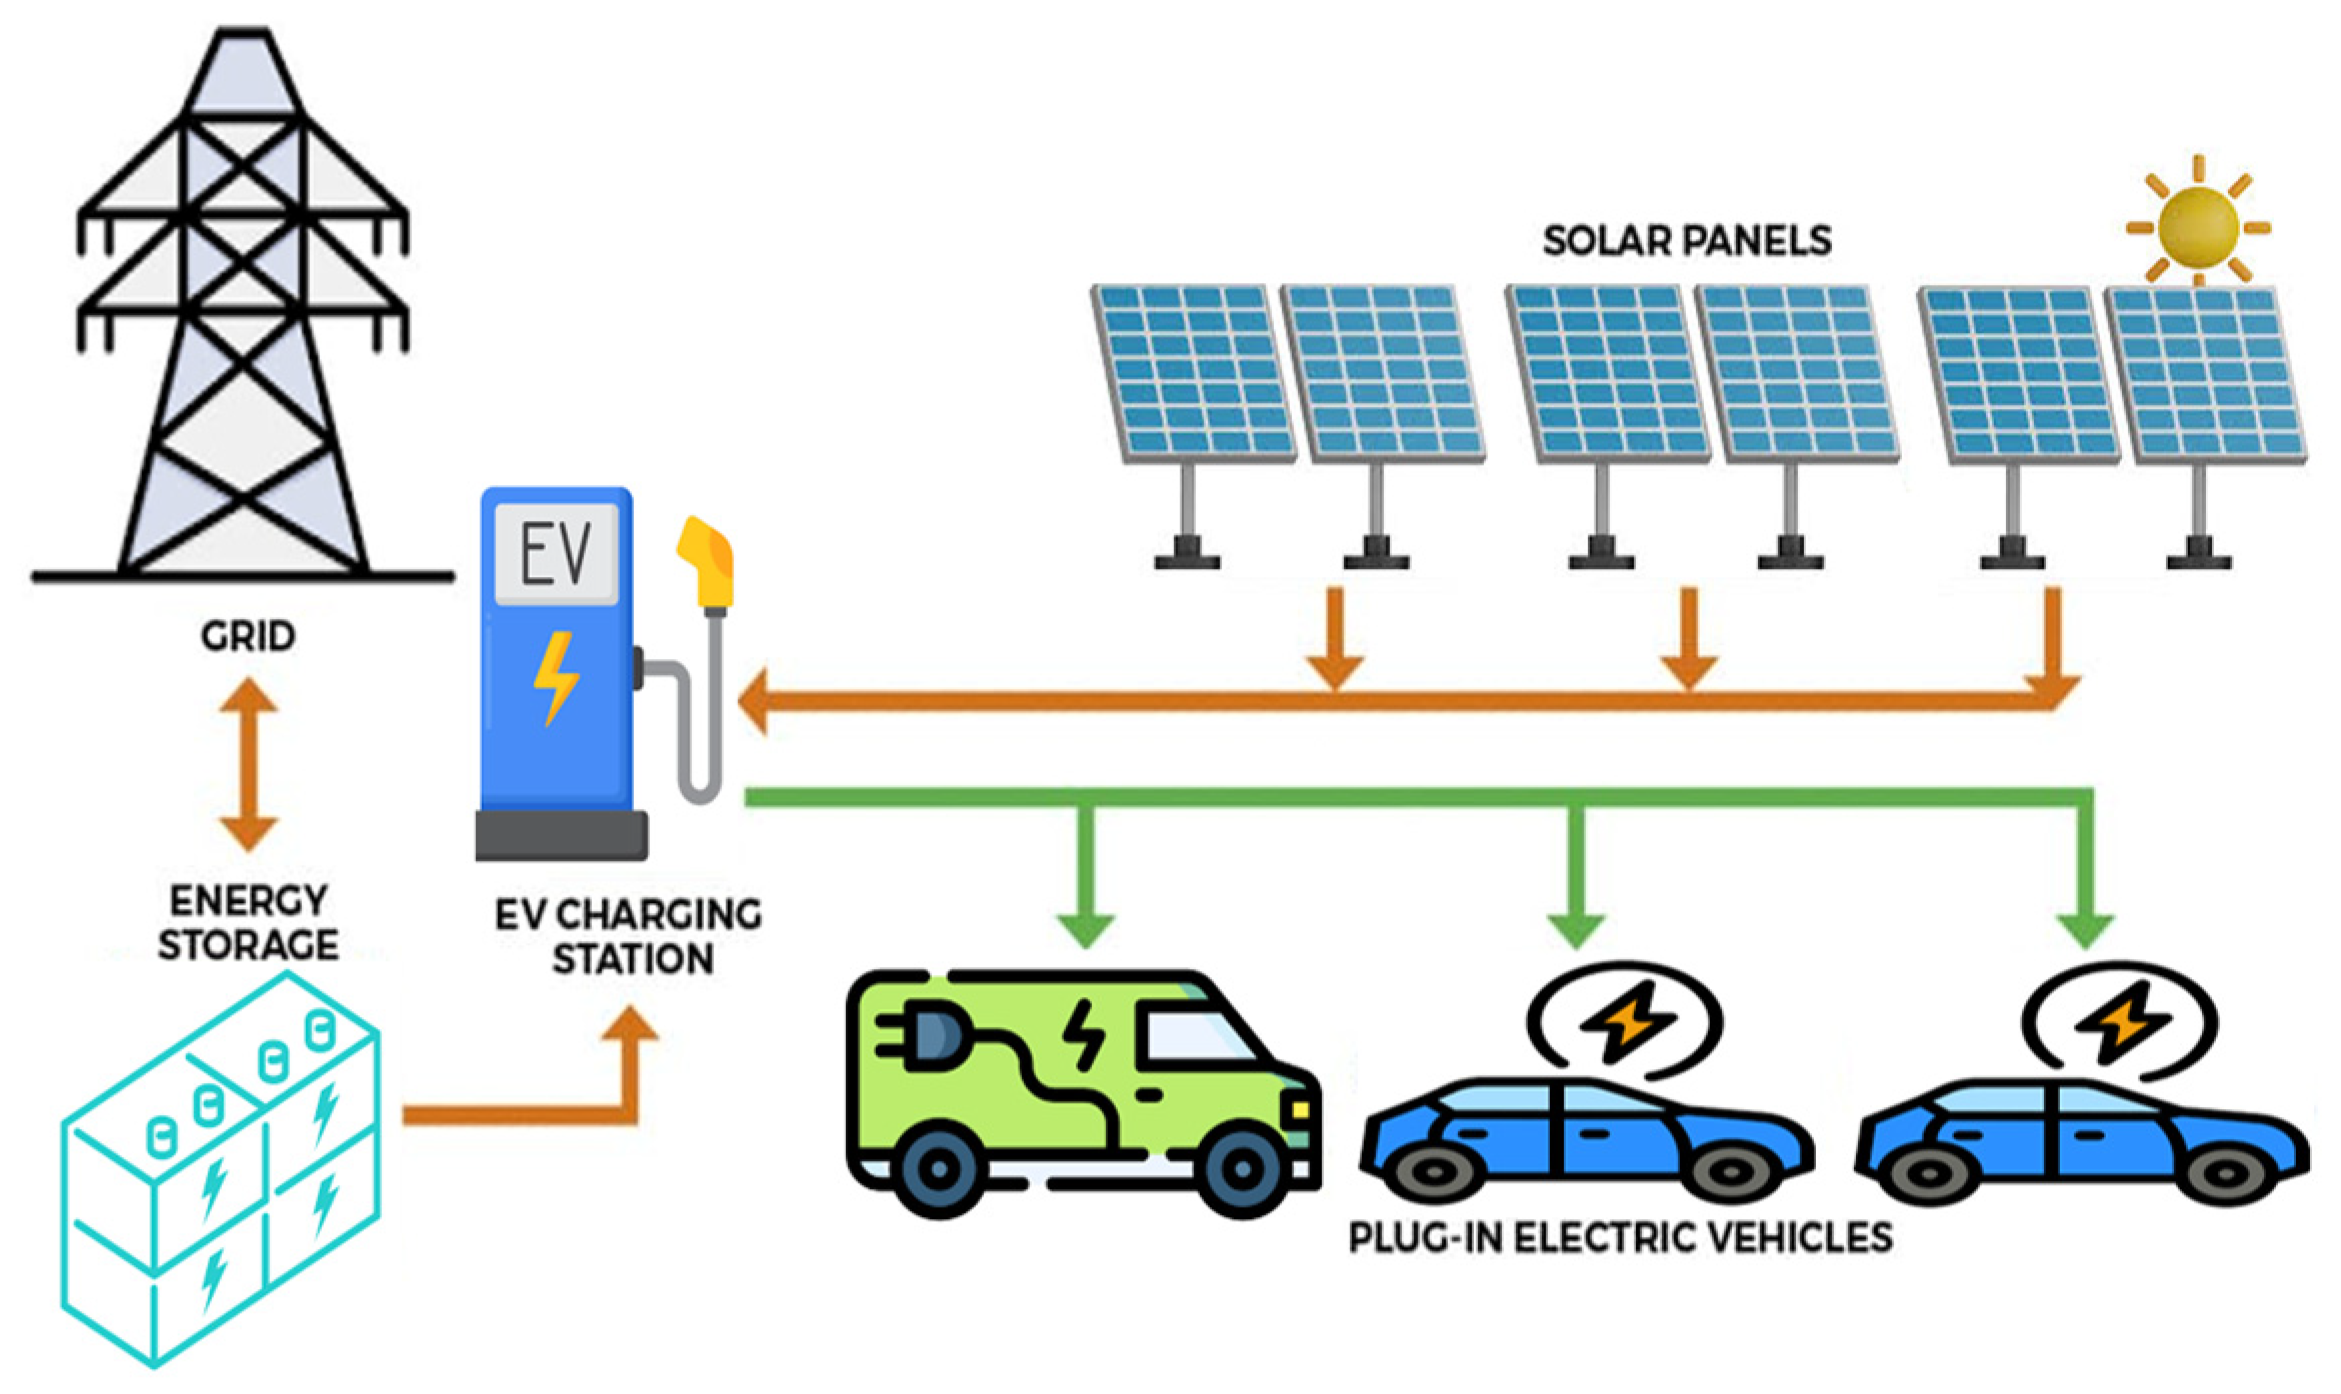
\includegraphics[width=0.6\textwidth]{Images/EVCI_diagram.png}
    \caption{\textbf{A typical EV charging infrastructure}~\cite{Deeum2023} \\Including electricity grid, 
    renewable generation (solar panels), energy storage systems, charging stations, 
    and plug-in electric vehicles. }
    \label{fig:EVCI_diagram}
\end{figure}

A typical EV charging infrastructure (EVCI) shown in Figure~\ref{fig:EVCI_diagram} highlights the importance of coordinating generation, storage, and charging to ensure reliable and sustainable operation. EVCI is both an enabler and a potential bottleneck of EV 
transition. Research highlights a persistent "chicken-and-egg" problem: users 
hesitate to purchase EVs without adequate charging coverage, while investors 
are reluctant to finance charging stations without a critical mass of EV users. 
Studies show that strategic deployment of charging points is more cost-effective 
than merely enlarging battery capacity, as infrastructure provision directly reduces 
range anxiety and supports large-scale diffusion~\cite{Metais2022}. 

From a planning perspective, charging infrastructure must address three 
dimensions: technical, economic, and user acceptance. Technical 
issues involve compatibility of charging standards, grid integration, and power 
demand management. Economically, the high costs of fast-charging stations 
require careful location and sizing strategies. User acceptance hinges on 
convenience, accessibility, and charging time, which significantly influence EV 
adoption~\cite{LaMonaca2022}. In summary, while EV adoption continues to expand rapidly, the success of the 
transition is inseparable from charging infrastructure. Planning, optimization, and 
digitalisation of charging networks will determine whether electrified transport 
can scale sustainably and equitably.

\subsection{Digital Twin and Simulation}

The increasing complexity of electric vehicle (EV) charging networks, 
their tight coupling with the power grid, and the variability of user 
behaviour make planning and operation challenging. Digital twin 
technology is increasingly viewed as a powerful tool to manage the complexity 
of charging networks, enabling real-time monitoring, scenario analysis, and 
integration with renewable power and storage systems~\cite{Yu2024}. A digital twin is defined as a ``live digital coupling of the state 
of a physical asset or process with a virtual representation that 
produces functional output''~\cite{Somers2023}.Figure~\ref{fig:DT_diagram} shows a typical EVCI. Unlike conventional 
models or static simulations, digital twins establish a continuous 
bi-directional link between the physical system and its digital replica, 
enabling real-time monitoring, predictive analytics, and feedback 
control~\cite{Liu2021Review,Enders2019}.

\begin{figure}[ht!]
    \centering
    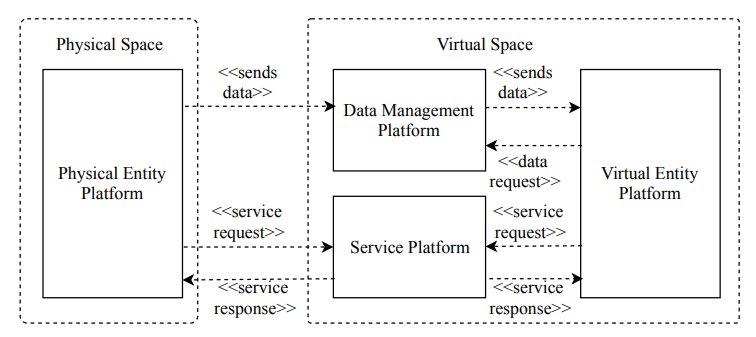
\includegraphics[width=0.7\textwidth]{Images/DT_diagram.png}
    \caption{\textbf{A Typical Digital Twin Framework}~\cite{8823809} \\
     A digital twin includes both physical and virtual space,with four components: Physical Entity Platform, Data Management Platform, Service Platform and Virtual Entity Platform.
}
    \label{fig:DT_diagram}
\end{figure}

In the context of EV charging infrastructure, digital twins offer 
several advantages. First, they enable multi-scale simulation of 
charging demand and grid interaction, supporting optimal siting and 
sizing of charging stations. Second, they allow scenario analysis under 
uncertainty, including stochastic EV arrivals and variable renewable 
generation, thereby enhancing grid stability and resilience~\cite{Talusan2024}. 
Third, digital twins provide a platform for testing cyber-physical 
interactions, including cybersecurity assessment, without disrupting 
operational systems~\cite{Eckhart2019}. These capabilities make digital 
twin frameworks particularly suitable for managing charging networks 
within smart cities and integrating them into future vehicle-to-grid (V2G) 
and vehicle-to-building (V2B) systems.

Simulation remains at the core of digital twin applications. Studies 
classify applications into \emph{simulation}, \emph{monitoring}, and 
\emph{control} purposes~\cite{Enders2019}. For EV charging, simulation 
provides the foundation to evaluate control strategies, optimize energy 
flows, and quantify environmental impacts. Discrete-event simulation 
platforms, such as OPTIMUS, extend these capabilities by integrating 
building energy use, grid events, and charging policies, allowing 
benchmarking of control algorithms under realistic conditions~\cite{Talusan2024}. 

\subsection{Data Models and Interoperability}

Digital twins function as high-fidelity virtual counterparts of physical systems, supporting real-time monitoring, simulation, and control. However, realizing their full potential hinges on seamless data interoperability—the ability of multiple systems to exchange, interpret, and act upon shared information. Without standardized representations, digital twin implementations often remain siloed, each relying on proprietary formats that limit aggregation and coordinated analysis across domains~\cite{David2024}. Addressing this fragmentation requires robust standards and transformation mechanisms to align heterogeneous digital twin models~\cite{Schmidt2023}.

\begin{figure}[ht!]
    \centering
    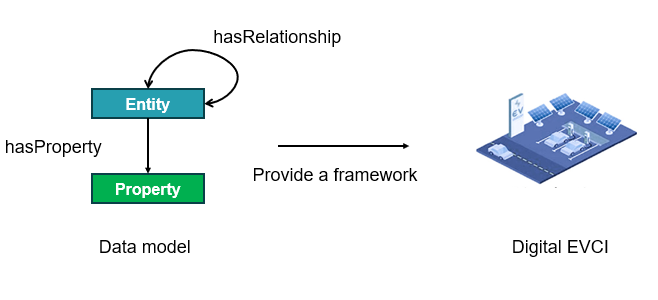
\includegraphics[width=0.65\textwidth]{Images/data-model.png}
    \caption{\textbf{From Data Model to Digital Twin}\\
    Data model is an abstract model that 
organizes and standardizes the relationships and properties of real-world entities. 
}
    \label{fig:data-model}
\end{figure}

Data models and ontologies play a crucial role in enabling interoperability. They provide a shared vocabulary and structure that allow systems to interpret information consistently across semantics, constraints, and behaviors~\cite{Karabulut2023}. Semantic technologies, knowledge graphs, and ontology-based integration frameworks are increasingly used to bridge modeling languages and domains, facilitating automated data fusion and richer collaboration between digital twins~\cite{Dunbar2022}. In addition, conceptual interoperability frameworks, such as those proposed by the Digital Twin Consortium, define atomic data entities and standardized messaging patterns to support modular composition of digital twins across system boundaries~\cite{Budiardjo2021}.

For infrastructures such as electric vehicle (EV) charging networks, interoperable data models are indispensable. They enable cross-system coordination between charging stations, grid services, and building energy systems; support automated integration of sensor data, user behavior, and energy flows; and provide a foundation for composable architectures where charging, storage, and renewable generation twins can interact within a unified ecosystem. Ensuring accurate, semantic-level interoperability is thus a prerequisite for building comprehensive, reliable, and scalable digital twin systems that can address the challenges of sustainable and intelligent mobility.
